%%% Local Variables:
%%% mode: latex
%%% TeX-master: t
%%% End:

\chapter{基于时间自动机的中断模型}
\label{cha:intr}

中断从出现发展到现在,尤其是在嵌入式开发领域的大量应用,其行为模式和实现方式也已
经有了很大的变化。现在在各个平台使用的中断也不再是单纯的一种简单模式,而是多种方
式并存。

\section{验证方案}
\label{sec:scheme}

为分析嵌入式程序里中断的实时性,本文的提出了一套完整的方案,分为以下五步:

首先,深入了解中断行为和背后的实现机制。模型构建必须建立在对目标行为的充分了解的基
础上。同时,了解中断背后的实现机制才能消除模型中一切可能的模棱两可的细节。并且,
充分了解实现机制可以为中断建模过程中的抽象和假设提供坚实的依据,保证模型的可靠性
和实用性。

第二,对中断做适度的抽象和假设。抽象和假设是为了简化问题,保证问题在后
续的研究中可解。在应用形式化方法时,这一步非常重要。经过该步,一个实际问题才能
转化为一个可以用形式化方法解决的问题。

第三,给出问题的形式化描述。这一步有助于帮助研究人员更精确地理解问题,同时也为后续的
形式化验证做好准备。

第四,构建合适的形式化模型。在这一步中,最关键是的理论本身的可靠性,理论对问题的
适应性,以及模型和原问题的一致性。三者缺一不可。例如在本文中,目前的时间自动机理
论对嵌入式程序的中断并不完全适用,因此本章对时间自动机理论做了扩展以适应问题。

第五,应用理论本身的相关技术进行分析和验证。针对本文,分析和验证时间自动机的模型
的技术就是模型检测。

应用此方法,本章从中断行为模式的角度,归纳常见的三种中断,并深入剖析他们的实现
方式。在构建中断模型时,本章首先进行抽象和假设,然后对中断给出形式化定义,最后
扩展时间自动机理论并给出对应的时间自动机网络的模型。由于本章并不涉及具体的问题,
因此实时性分析一步在本章未有体现,请参见第~\ref{cha:case} 章的应用。

\section{中断机制}
\label{sec:intr_machanism}

按照行为模式的不同,本章将中断分为\textbf{基本中断},\textbf{可重入中断}和
\textbf{分段中断}三个类型。

\subsection{基本中断}
\label{subsec:basic}

通常,在我们接触到的非实时性桌面电脑环境中的中断就是一个本章所述的基本中断。

\subsubsection{基本中断的行为}
\label{subsubsec:basic_behavior}

基本中断的行为模式是简单的抢占当前线程,在执行结束之后恢复上下文继续执行被抢占的
线程。

\begin{figure}[H]
	\centering
	
\includegraphics[width=0.4\textwidth]{thread_states}
	\caption{单个线程的状态}
	\label{fig:thread_state}
\end{figure}

中断处理程序的行为,与多线程程序研究中的线程行为十分相似。我们对中断模型的构建就
参考了多线程程序中的线程模型。如图~\ref{fig:thread_state} 所示,通常,一个线程
会被刻画为以下三个状态。

\begin{itemize}
	\item \emph{就绪}:线程可以运行但是当前并不占有CPU。
	\item \emph{运行}:线程正在运行。
	\item \emph{阻塞}:线程在等待处理器以外的资源,暂时无法运行。
\end{itemize}

由于绝大部分多线程程序研究的场景中,并不关心线程产生和终止。换言之,线程在这类应
用场景里直接存在,且永不终止。中断研究中,一个中断通常具有一个从产生到终止的完整周期
。而且,一个中断并非只触发一次,因此一个可能重复多次上述周期。这与传统的多线程程
序研究是不同的。所以针对一个,我们类比线程再加以修改可以得到如图~\ref{fig:interrupt_state} 
所示的状态机。每个状态的含义如下。

\begin{figure}[H]
	\centering
	
\includegraphics[width=0.4\textwidth]{interrupt_states}
	\caption{单个中断的状态}
	\label{fig:interrupt_state}
\end{figure}

\begin{itemize}
	\item \emph{无中断}:当前中断没有触发。
	\item \emph{就绪}:中断触发但是有优先级更高的中断在执行。
	\item \emph{运行}:正在运行。
	\item \emph{阻塞}:被优先级更高的中断打断。
\end{itemize}

\begin{figure}[H]
	\centering
	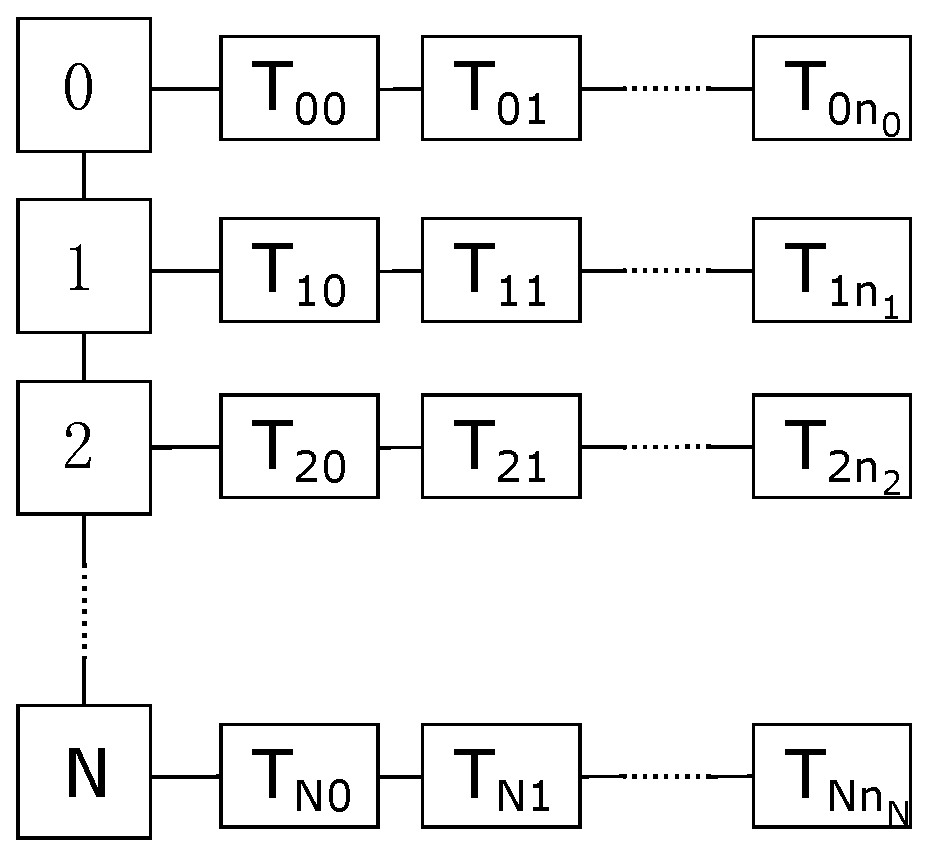
\includegraphics[width=0.5\textwidth]{thread_table}
	\caption{线程表}
	\label{fig:thread_table}
\end{figure}

在多线程的场景中,线程之间的切换往往由线程调度器掌管。线程调度器不是硬件,而是一
段代码,负责实现线程之间的调度。时间片轮转,优先级不同的线程之间的抢占,甚至是线
程优先级的动态变化,都由线程调度器实现。一般而言,线程调度器是系统内核的重要组
成部分。线程调度器工作的基础就是如图~\ref{fig:thread_table} 所示的线程表结构。
线程表通常是一个二维的表,由系统所支持的线程优先级数构成表的行,每一行内是属于该
优先级的所有线程。通常情况下,系统中会有一个就绪线程表和一个阻塞线程表,当前线程
不在任何一个表中。所有的线程调度算法其实都是对这个表的调整。

相比而言,多中断场景比多线程场景简单许多。通常情况下,一个中断优先级对应一个中断
处理程序。所以,中断处理程序的组织形式也是一个表,但是从二维降到了一维。在大部分
文档中,这个表被称为中断向量表(Interrupt Vector Table),如图~\ref{fig:interrupt_vector_table} 
所示。中断向量表中的每个表项被称为一个中断向量(Interrupt Vector),指代一个中
断处理程序。在实现时,一个中断向量通常是一个函数指针,指向某个函数,该函数的内容
就是中断处理。因此,不同于多线程场景中,一个线程优先级可以对应多个线程,一个中断
优先级对应最多一个中断。中断优先级是由CPU或外部中断控制器等硬件决定的,实际使用
时可能用不到所有的优先级,因此会有大量的中断向量表项为空。

\begin{figure}[H]
	\centering
	
\includegraphics[width=0.2\textwidth]{interrupt_vector_table}
	\caption{中断向量表}
	\label{fig:interrupt_vector_table}
\end{figure}

除了维数降低,中断向量表相比于线程表而言,还有两个不同点。

其一,一般而言,中断向量表在系统初始化完成以后就不再变化。这里的变化指的是已有的
中断的优先级变化,即已有中断在中断向量表中的位置变化。部分操作系统或裸机程序会有
在运行时注册或注销中断的行为,但是从来没有过更改一个现有中断优先级的行为。换言之,
在运行时,中断向量表可以增加或删除表项,但不会更改表项。\footnote{这是一条编程
准则。事实上,只要有足够的权限,更改中断向量表项的操作是被允许的,因而也是可以完
成的。只不过大家都不这么做。}

其二,中断向量表只有一份,包含了所有的中断,不论其当前状态如何。以线程表而言,系
统中可能有两份甚至多份线程表,分别记录不同状态下的线程。除了笼统地将阻塞线程做成
一张线程表,还有一些实现是将请求同一个锁变量的阻塞线程做成一张单独的表。在该实现
下,系统内会同时存在$L+1$张线程表($L$代表系统中锁的数量),另外还有一个当前线程
不在任何线程表内。

到此,一个概念中最基本的中断模型就形成了。中断处理程序状态机如图~\ref{fig:interrupt_state} 
所示,中断向量表如图~\ref{fig:interrupt_vector_table} 所示。

\subsubsection{基本中断的实现}
\label{subsec:basic_hardware}

中断的实现最主要两个部分是的中断控制器和中断向量表。

中断控制器在硬件实现上可以是一个包含控制线路的独立系统,也可以被集成进存储器子系
统中。对于前者,在IBM个人机上,广泛使用可编程中断控制器(Programmable Interrupt 
Controller,PIC)来负责中断响应和处理。PIC被连接在若干中断请求设备和处理器的中断
引脚之间,从而实现对处理器中断请求线路(多为一针或两针)的复用。作为另一种中断实
现的形式,即存储器子系统实现方式,可以将中断端口映射到存储器的地址空间,这样对特
定存储器地址的访问实际上是中断请求。一般桌面领域的PC机中,中断控制器一般是集成在
处理器内部,而在嵌入式领域,很多厂商推出的微控制器实现了外置的中断控制器。
\footnote{例如Intel的8086系列处理器提供了内置的中断控制器,而意法半导体
(STMicroelectronics)推出的STM32F4系列微控制器中,在ARM的CPU外提供了中断控制器。}

无论是CPU内部还是外部的控制器,其控制逻辑都是类似的。通常,CPU会有一个或多个指示
当前各种状态的STATUS寄存器。STATUS寄存器中有一位表示是否有中断需要处理,我们称其
为中断标志位。CPU在每一个指令周期之后会检查中断标志位是否置位,如果置位,CPU会和
中断控制器通信获取中断号,然后保存当前上下文,即将上下文压栈,如图~\ref{fig:stack} 
所示。注意,上下文的具体内容视不同硬件平台决定,图中只作示意。程序计数器(
PC)加载中断向量表中对应表项所指向的中断处理程序地址,开始执行中断程序。进入中断
处理时,CPU还会修改STATUS寄存器中的其他的位以表示它现在正在处理中断。相应的,中
断控制器上会有寄存器指示当前所有的中断的状态。在接受新的中断触发信号之后,中
断控制器内部的判定逻辑会决定该中断是否可以立即抢占CPU,进而决定是否需要将CPU的
STATUS寄存器中的中断标志位置位。

相对于中断控制器,中断向量表的实现逻辑简单许多。通常,中断向量表是在内存中一块
独立的区域。在许多平台上,这块
区域从0x0000\footnote{这里用16位数只是举例,表示在内存首地址。如果在32位或64位
平台,地址应该写成0x0000 0000或0x0000 0000 0000 0000}开始。CPU会根据一个
中断向量号来查找对应表项,而中断向量表的基地址完全由CPU的硬件实现规定。部分CPU
允许在系统初始化的时候重新选择中断向量表的基地址,其原理就在于在这些CPU寻址中断
处理程序时,中断向量表基地址是从一个内部寄存器中取出。通过特定的汇编语句可以修改
该寄存器的值。在硬件上电启动之前,中断向量表里
的表项并未被赋值。上电之后,在初始化时,由软件给中断向量表各个用到的表项填上对应
的值,通常是各中断处理函数的函数指针。

\begin{figure}[H]
	\centering
	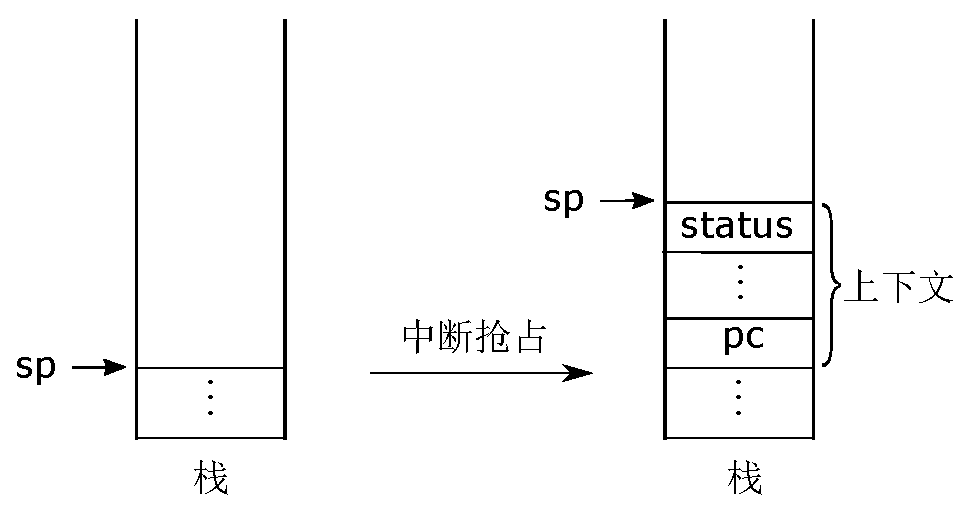
\includegraphics[width=0.7\textwidth]{stack}
	\caption{中断发生前后的栈变化}
	\label{fig:stack}
\end{figure}

\subsection{可重入中断}
\label{subsec:reentrant}

在~\ref{subsubsec:basic_behavior}小节中,我们说到中断会被更高优先级的中断打断,
低优先级的中断到来之后也只有等待高优先级的中断执行完才能得到CPU资源。那么如果一个
中断在执行时,有一个同优先级的中断触发了,或者更准确的表述是,一个中断的某一个实
例在运行时,它的下一个实例触发,这时,新来的中断实例应该进入就绪状态等待。然而,
事实上,很多应用场景里,会要求同优先级的中断也可以打断当前中断。如果某中断的下一
个实例能够抢占前一个实例,我们就称该中断支持重入(re-entrance)。许多中断平台现
在已经支持中断重入,也有许多软件产品使用了中断重入这个特性。

\subsubsection{可重入中断的行为}
\label{subsubsec:reentrant_behavior}

从我们对重入的定义可以看出,可重入中断的本质在于同中断的下一个实例可以打断当前实例, 
其行为也如~\ref{fig:interrupt_state} 所示,只不过从运行到阻塞状态也可以由当前
中断的下一个实例触发。

\subsubsection{可重入中断的实现}
\label{subsec:reentrant_hardware}

可重入中断的实现与~\ref{subsec:basic_hardware} 小节中描述的基本中断
的通用实现基本相同,差别仅在于中断控制器的优先级判定规则。

如果我们从栈(Stack)的角度来看中断重入,会发现重入与非重入的抢占在栈的行为上是
完全一致。在~\ref{subsec:basic_hardware} 小节中我们描述了中断抢占发生时上下文
会被压栈。重入时栈上的行为与图~\ref{fig:stack} 完全一致。由此可见,重入的次数没
有任何理论上的限制。即同一个中断的任意多个实例都可以连续到来,并打断前一个实例。
但是,在真实的硬件平台上,因为栈的大小受到内存容量的约束,重入的次数受栈大小的限
制,所以重入的次数实际上总有一个上界。\footnote{这也是中断嵌套的层数限制,本质上
与中断是否重入没有关系。}

\subsection{分段中断}
\label{subsec:segment}

分段中断,顾名思义,就是中断并非一次执行,而是分成两段或者多段\footnote{目前尚未
见到将中断分为多段的案例}执行。这个划分是中断机制主动为之,而非被其他中断抢占CPU
而被动分段执行。即,在本中断当前优先级最高的前提下,本中断仍然会分段执行。

\subsubsection{分段中断的行为}
\label{subsubsec:segment_behavior}

在实际应用中,中断的行为并不一直忠实地遵从其硬件实现,操作系统可以在一定程度上改
变中断的行为。在嵌入式操作系统中,出于实时性的考虑,一个中断的运行时间不应该过长,
但是许多中断需要实现的逻辑功能却比较复杂。因此一个通用的解决方案就是在操作系统中
将中断分成两段,前一段在中断触发时立即执行,后一段则延后执行。后一段代码的执行优
先级较低,因此有可能被其他低优先级中断甚至是普通代码抢先执行。这样,在编写中断代
码的时候,将需要立即执行不容延迟同时运行时间较短的代码放在第一段,其他的对延时不
敏感,或者任务繁重,或者需要和其他线程进行同步交互的代码放在第二段,就能在满足实
时性要求的前提下完成该中断。eCos等部分操作系统尽管实现方式各异,采用的都是分段中
断的模式。\cite{ecos}图~\ref{fig:intr_exec} 和图~\ref{fig:ecos_intr_exec} 分
别展示了两种中断的执行流。

\begin{figure}[H]
	\centering
	\subcaptionbox{普通中断的执行流\label{fig:intr_exec}}
	{
\includegraphics[width=0.3\textwidth]{interrupt_exec_model}}
	\hspace{4em}%
	\subcaptionbox{分段中断的执行流\label{fig:ecos_intr_exec}}
	{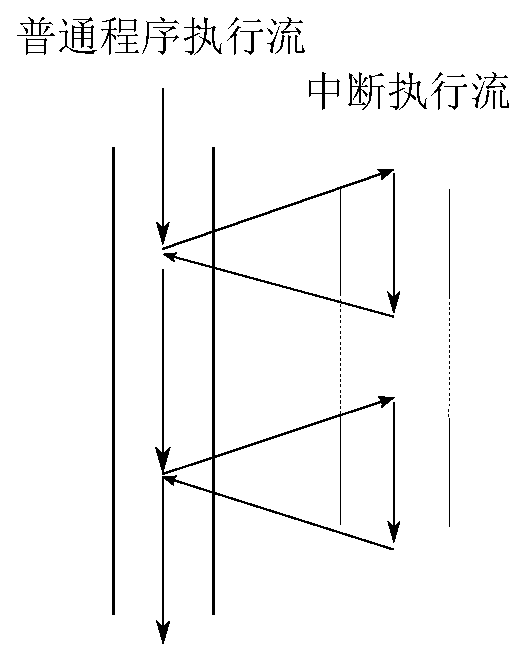
\includegraphics[width=0.3\textwidth]{ecos_interrupt_model}}
	\caption{不同的中断执行流}
	\label{fig:two_intr_exec}
\end{figure}

分段中断的出现从嵌入式开发的角度来讲,极大地方便了应用的开发,可以在不牺牲实时性
的同时让中断完成更繁重的任务。这一点在开发中断驱动程序(Interrupt-driven Program
)的时候极为重要。中断驱动程序的主要功能都是在中断中完成。如果功能比较复杂或者牵
涉到与其他硬件的交互,不可避免地,中断处理时间会比较长。在没有分段处理的情况下,
低优先级的中断的响应时间将大为增加,实时性无法保证。

\subsubsection{分段中断的实现}
\label{subsubsec:segment_software}

分段中断的行为看起来很美好,但是这有悖于我们对中断机制一直以来的理解。正如上文所
说,分段中断是操作系统系统的二次实现。这也是为了实现实时性需求嵌入式开发程序员在
硬件平台不支持分段中断的情况下做出的机智创作。市面上多家实时操作系统提供了分段中
断的机制。在此以eCos操作系统为例介绍分段中断机制。

eCos是一个跨平台的操作系统,支持各类CPU和板载中断控制器。不同平台对应的汇编代码
并不一样,在此我仅以ARM提供的Cortex M系列CPU为硬件平台讲解eCos的分段中断机制。
为了使读者能够理解我将要描述的实现细节,首先我会对Cortex M系列CPU跟中断处理相关
的内容做简要介绍。

Cortex M系列CPU采用ARMv7-M体系结构,该体系结构针对移动平台设计,在能耗上相当好
的控制。在中断\footnote{在ARMv7-M Architecture Reference Manual中,ARM称本文
所说的中断为异常(Exception),其中,0-15号异常为预定义好的,其处理程序也已固化
在硬件上,16号以后的异常被称为中断(Interrupt)。这只是术语的不同,为了防止混淆,
在本文中统称中断(Interrupt)。}控制机制上,ARMv7-M体系结构与~\ref{subsec:basic_hardware}
小节所述类似,也采用在栈上保存上下文,进入中断处理之后结束再恢复上下文。

ARMv7-M体系结构包含13个通用寄存器,R0-R12,以及3个额外的特殊寄存器。

\begin{description}
	\item[SP] 栈指针,用来指示当前活跃的栈的顶部内存位置。SP有时也被称为
	R13。
	\item[LR] 链接寄存器,用来保存返回链接。返回链接是指进行了一次带返回
	的跳转指令的返回地址,通常是跳转指令的下一条指令。该寄存器的复位值为0xFFFFFFFF,
	使用该值进行跳转返回会触发一个错误。LR寄存器在进入中断时也会更新,我们会在
	下文描述。LR有时也被称为R14。
	\item[PC] 程序计数器。PC有时也被称为R15。
\end{description}

在ARMv7-M体系结构中,内存中同时存在两个栈空间\pozhehao 进程栈和主栈,进程栈属
于当前线程,主栈则是所有程序共用。尽管每个线程都有一个自己的进程栈,但是SP所指
向的进程栈是当前进程栈。CPU内有两个特殊寄存器。

\begin{description}
	\item[PSP] 进程栈指针,永远指向当前进程栈的栈顶。
	\item[MSP] 主栈指针,永远指向主栈栈顶。
\end{description}

SP的读取值可以是PSP的值也可以是MSP的值,即PS可以指向当前进程栈栈顶也可以指向主
栈栈顶,这取决于专用CONTROL寄存器的SPSEL位(即第1位)的当前值。如果为CONTROL.SPSEL
的值为0,SP指向主栈栈顶;如果CONTROL.SPSEL的值为1,SP指向进程栈栈顶。CPU有线
程模式(Thread Mode)和处理模式(Handler Mode),在线程模式下,CONTROL.SPSEL
的取值可以是0或1;在处理模式下,CONTROL.SPSEL的读取值永远为0。换句话说,在线程
模式下,SP可以指向进程栈或主栈,但是在处理模式下,SP永远指向主栈。CPU在接收中断
时会进入处理模式。在处理模式中,CPU可以使用psp和msp在汇编代码里直接操作对应的栈。

在CPU接收到中断信号的,它会将8个32为寄存器压栈,包括xPSR寄存器,返回地址,LR,R12,
R3,R2,R1和R0。这与CPU在执行函数调用时遵守的ARM Architecture Procedure Calling
Standard(AAPCS)保持一致。在进入中断时,LR会被写入一个特殊的值\textbf{EXC\_RETURN}。
因为返回地址和LR原本的值都已经被压栈保存起来,因此LR在中断处理时空闲出来。中断处理
时,返回的标志就是向PC寄存器中写入EXC\_RETURN。一般情况下,写入的EXC\_RETURN就是
LR中保存的值,也可以是从其他途径得到的值。EXC\_RETURN的取值固定且分别具有不同的含
义,如表~\ref{tab:exe_return_noFP} 和表~\ref{tab:exe_return_FP} 所示。在
表~\ref{tab:exe_return_FP} 中的帧类型是指浮点数扩展模式下触发中断时压入栈的寄存器
构成的帧类型。有无浮点数支持,上述8个寄存器都会被压栈,且接下来的分析也只需要用到
它们,因此浮点数的模式在此不做单独讨论。\cite{ARM} 

\begin{table}[htb]
	\centering
	\caption{EXC\_RETURN定义的中断返回行为,无浮点扩展}
	\label{tab:exe_return_noFP}
	\begin{tabularx}{\linewidth}{XXX}
		\toprule[1.5pt]
		{\heiti EXC\_RETURN} & {\heiti 返回到模式} & {\heiti 返回到栈}\\
		\midrule[1pt]
		0xFFFFFFF1 & 处理模式 & 主栈 \\
		\midrule[0.5pt]
		0xFFFFFFF9 & 线程模式 & 主栈 \\
		\midrule[0.5pt]
		0xFFFFFFFD & 线程模式 & 进程栈 \\
		\bottomrule[1.5pt]
	\end{tabularx}
\end{table}

\begin{table}[htb]
	\centering
	\caption{EXC\_RETURN定义的中断返回行为,有浮点扩展}
	\label{tab:exe_return_FP}
	\begin{tabularx}{\linewidth}{XXXX}
		\toprule[1.5pt]
		{\heiti EXC\_RETURN} & {\heiti 返回到模式} & {\heiti 返回到栈} &
		{\heiti 帧类型}\\
		\midrule[1pt]
		0xFFFFFFE1 & 处理模式 & 主栈 & 扩展\\
		\midrule[0.5pt]
		0xFFFFFFE9 & 线程模式 & 主栈 & 扩展\\
		\midrule[0.5pt]
		0xFFFFFFED & 线程模式 & 进程栈 & 扩展\\
		\midrule[0.5pt]
		0xFFFFFFF1 & 处理模式 & 主栈 & 基本\\
		\midrule[0.5pt]
		0xFFFFFFF9 & 线程模式 & 主栈 & 基本\\
		\midrule[0.5pt]
		0xFFFFFFFD & 线程模式 & 进程栈 & 基本\\
		\bottomrule[1.5pt]
	\end{tabularx}
\end{table}

以上便是Cortex M系列CPU与中断相关的硬件规定,接下来我们详细讲解eCos的分段中断实现。

应用程序在注册中断时,需要提供两段程序,分别称为ISR(
ImmediateService Routine)\footnote{注意与本文其他章节里的中断服务寄存器ISR区分,
在本小节中涉及的的所有ISR均指代Immediate Service Routine。}和DSR(Delayed Service 
Routine)。其中,ISR在中断触发之后立即被执行的(如果优先级满足条件的话),DSR则
会被推迟执行,所有DSR的优先级低于一切ISR,所有DSR之间的优先级是同等的。\cite{ecos_isr}
经过对eCos代码的研读分析,如果在中断触发时,ISR执行完之后,DSR因故未能执行,那么
所有的DSR会在下一次线程切换时全部执行完毕。这样的好处是显而易见的。应用程序将必须
立即处理的不涉及共享资源或者运行时间比较短的部分放在ISR中处理,把剩下的部分放在DSR
里,既充分利用中断的便利,又不牺牲程序的实时性性能。\footnote{值得一提的是,应用
程序并没有选择使用传统的一段式中断的自由。在逻辑上,程序员只能把所有中断代码放在
ISR中,并提交一个空的DSR来完成传统的一段式中断的行为。此时,操作系统在此因为DSR的
处理反而会消耗相比传统一段式中断更多的CPU周期。}

%Let them flow
\begin{figure}
	\centering
	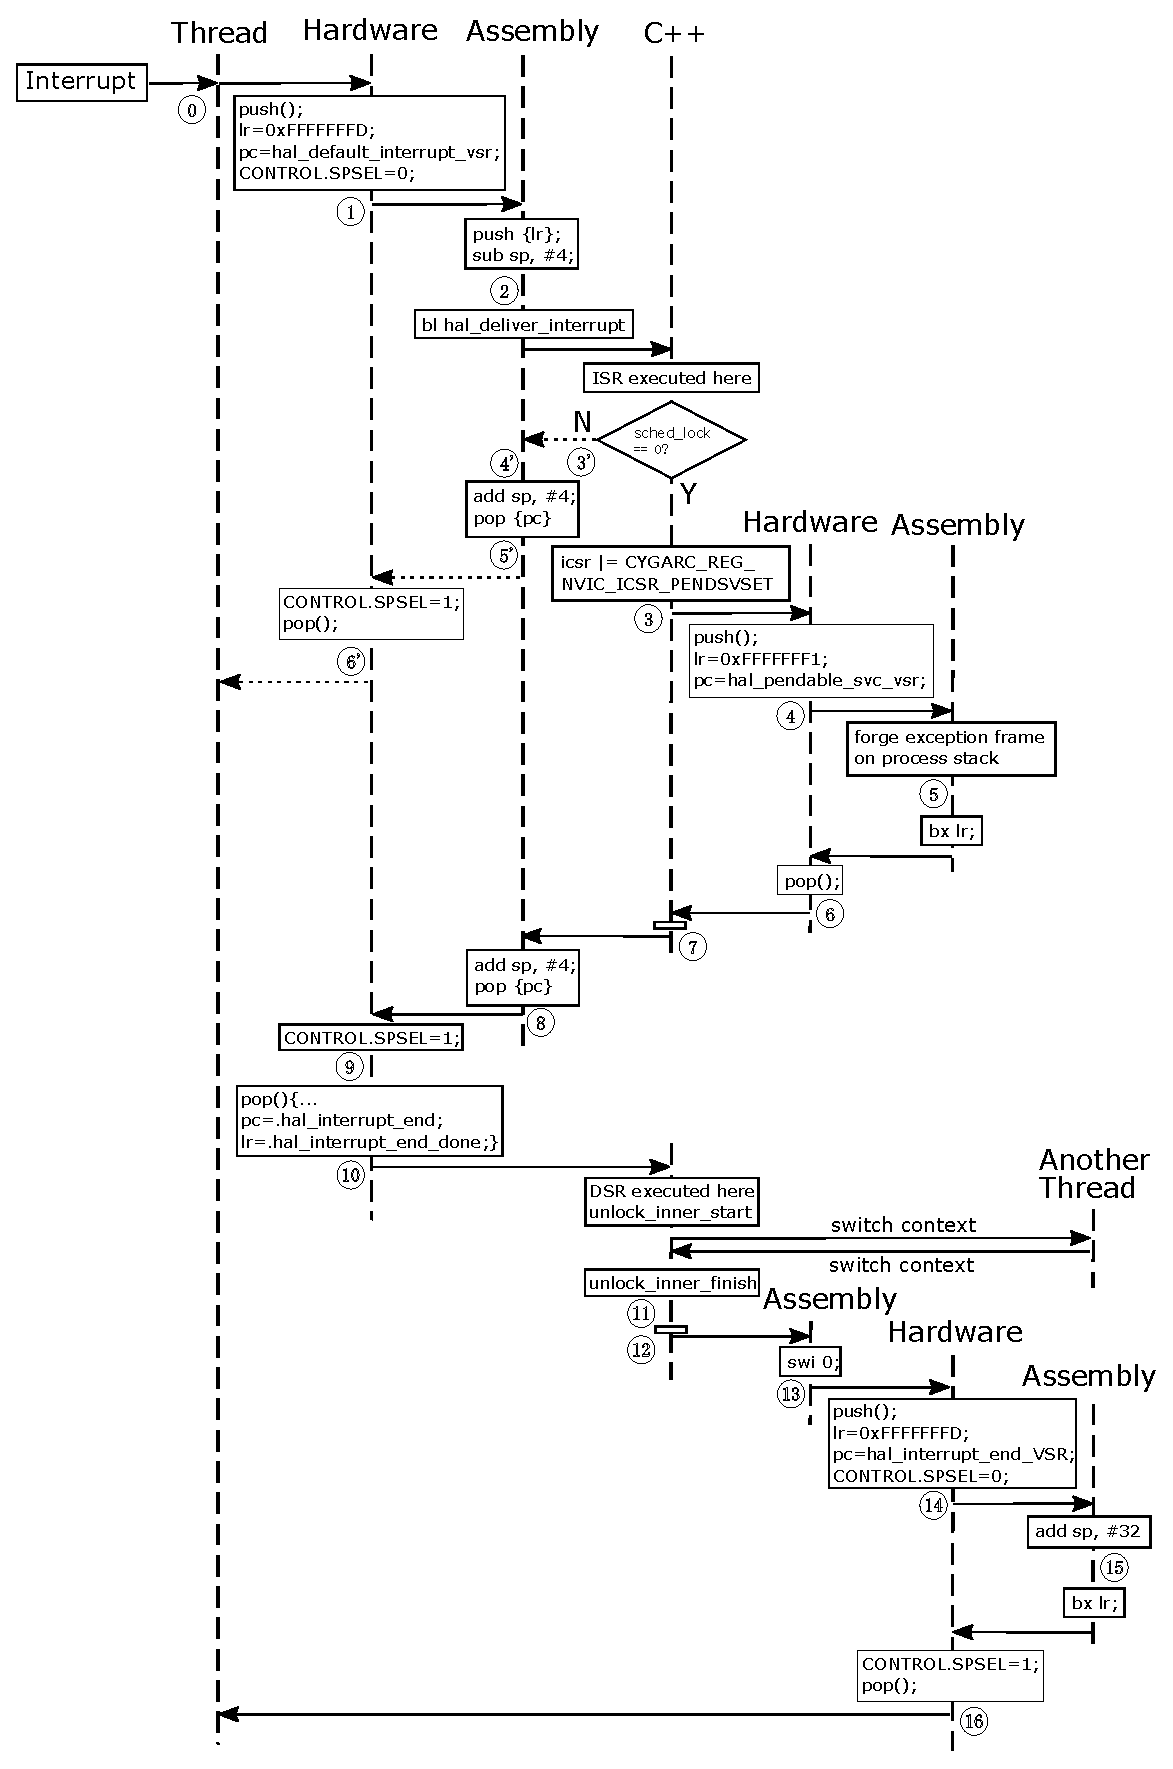
\includegraphics[width=\textwidth]{ecos_isr_dsr}
	\caption{eCos分段中断图解}
	\label{fig:ecos_isr_dsr}
\end{figure}

\begin{figure}
	\centering
	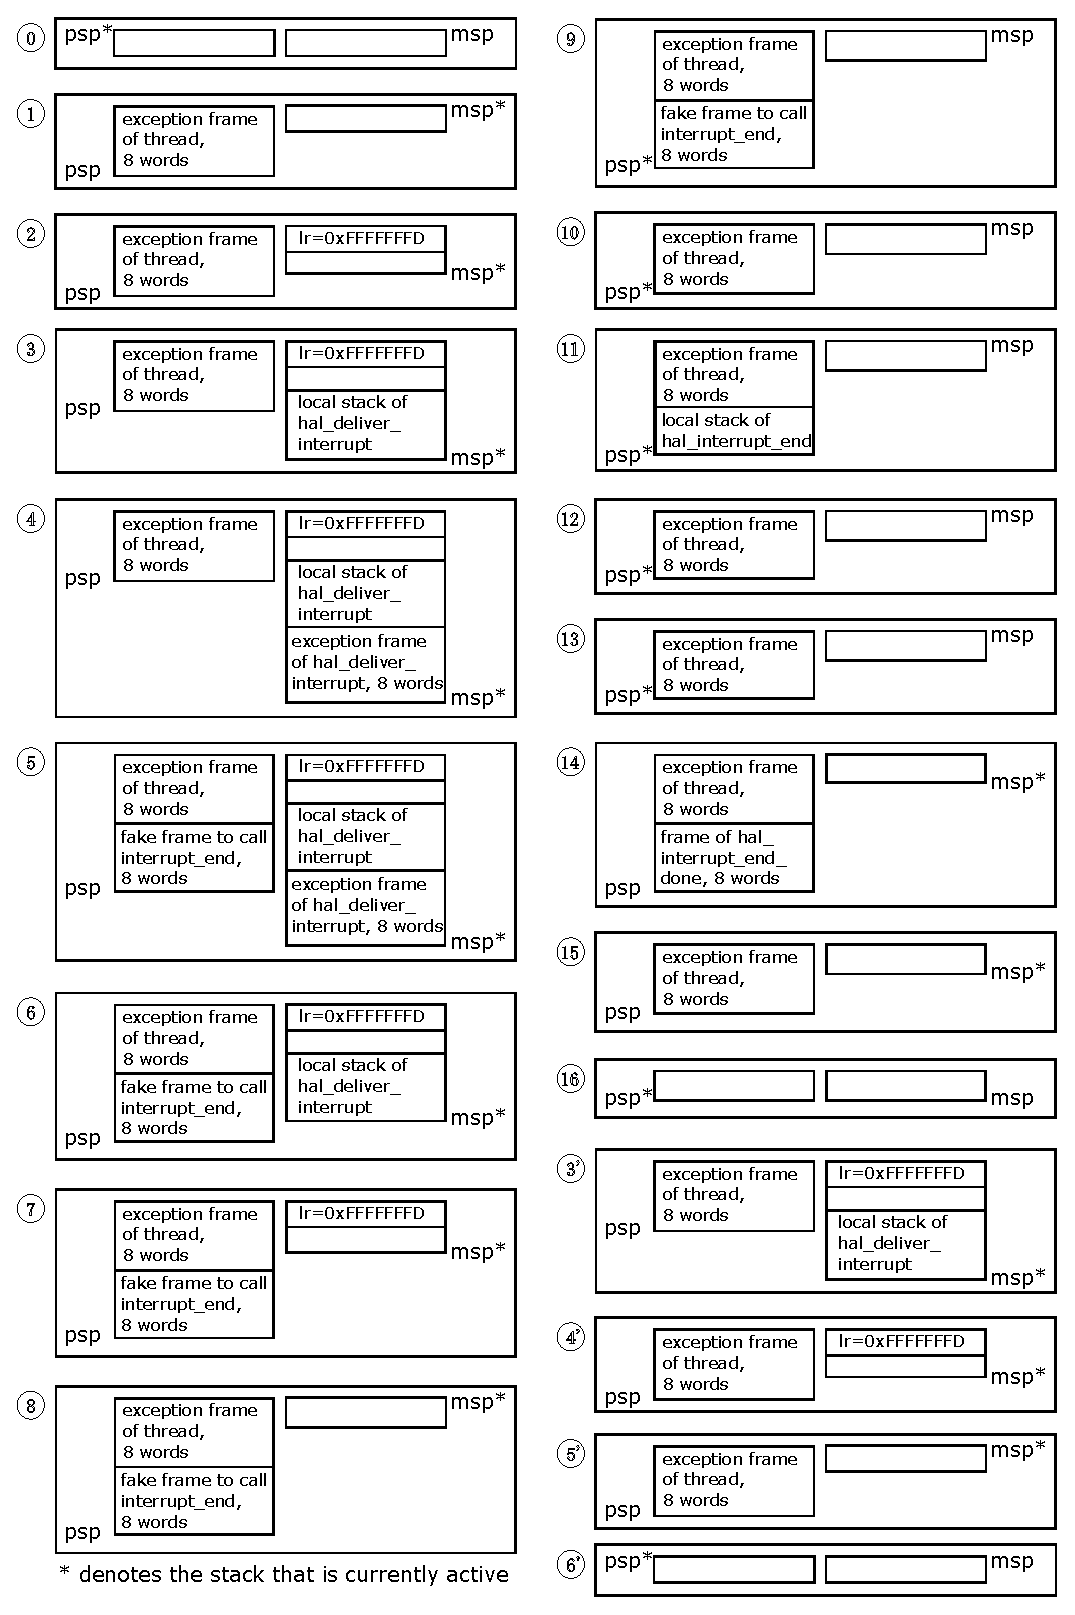
\includegraphics[width=\textwidth]{ecos_stack}
	\caption{eCos分段中断栈情况一览}
	\label{fig:ecos_stack}
\end{figure}

经过对eCos内核和针对Cortex M系列CPU的HAL(Hardware Abstract Layer, 硬件抽象层)
代码的仔细研读,我们将eCos操作系统的分段中断流程整理成图~\ref{fig:ecos_isr_dsr} 。
各个标号位置的栈情况见图~\ref{fig:ecos_stack} 。下面我们按照图示详细剖析一遍。

首先,CPU检测到中断信号,打断了当前线程。在位置0,我们可以看到主栈和进程栈同为
空\footnote{这里忽略检测到中断信号之前的栈内的内容,且不考虑栈溢出的情况。},且
当前活跃栈为进程栈。从位置0到位置1,是硬件接收中断的行为,这里最主要的是保存8个
32位寄存器(即程序上下文),将lr赋值为EXC\_RETURN,将PC定位到中断向量表项,即
hal\_default\_interrupt\_vsr的地址,以及CONTROL.SPSEL复位,即从位置1开始,活
跃栈切换为主栈。位置1之后的汇编代码就属于hal\_default\_interrupt\_vsr,首先将
lr的值压栈,然后将栈顶指针减4,即让栈涨了一个字,然后执行bl指令跳转到
hal\_deliver\_interrupt函数,因为bl指令是带返回地址的跳转至零,因此执行bl会将返
回地址写入lr寄存器中。不过在此之前lr的值已经被压栈了,如位置2的栈情况所示。
hal\_deliver\_interrupt是一段C++的函数。首先它完成了ISR的功能,接着会检查sched\_lock
这个变量的值。sched\_lock是定义在eCos系统的内核部分的一个关键变量,该变量指示是
否能进行线程调度,导致该变量为非0值的可能原因有很多,均需要CPU尽可能快的处理,因
此在sched\_lock不为0时,DSR就会被延后执行,本次中断处理就准备收尾了。在
图~\ref{fig:ecos_isr_dsr} 中,从位置3'开始,位置4',5',6'组成了一条退出中断的
路径。在汇编代码,即hal\_default\_interrupt\_vsr的后半部分,栈顶退回一个字的大
小,然后将栈顶的值,即进入hal\_default\_interrupt\_vsr时的lr的值,也就是进入中
断时存入lr的EXC\_RETURN写入pc寄存器,触发一个退出中断的硬件行为。硬件将
CONTRL.SPSEL根据EXC\_RETURN恢复为1,然后将保存的上下文恢复。本中断结束。位置6'
与位置1的栈情况完全相同。

另一方面,如果sched\_lock为0,eCos会去继续执行DSR。但是此时依然是在中断状态,如
果将DSR直接放在hal\_deliver\_interrupt里,它的优先级依旧高于其他低优先级的中断,
为了使所有中断的优先级高于DSR,我们需要在非中断状态执行DSR。接下来所做的复杂工作
就是为了去非中断状态执行DSR,然后再恢复上下文回到中断触发时的状态。

在判断sched\_lock为0之后,hal\_deliver\_interrupt将一个特殊的值CYGARC\_REG\_NVIC\_
ICSR\_PENDSVSET写入icsr寄存器,将中断检测位置位,CPU检测到一个新的中断,引发进
入中断的硬件行为。注意,这是一个中断嵌套,因为前一个中断尚未退出。类似的,硬件保
存上下文,在lr中写入EXC\_RETURN,修改pc到中断向量表项。然后就跳转到这个中断的处
理程序,即用汇编代码写的hal\_pendable\_svc\_vsr过程。在hal\_pendable\_svc\_vsr
中,eCos在进程栈里伪造了一个8个字的中断帧。然后利用bx指令将lr里的值,即
EXE\_RETURN写入pc寄存器,从而触发一个硬件的退出中断的行为。硬件在位置6恢复了位置3
的上下文,包括主栈和对应的寄存器。但是,我们注意到,位置6的进程栈里多了伪造的中断帧。

从位置7回来之后,hal\_deliver\_interrupt函数就结束了。C++的函数结束时,会从活跃
栈中弹出对应内容到寄存器里,将栈空间和寄存器都还原到进入函数之前的状态。\cite{AAPCS}
接着,CPU继续执行汇编过程hal\_default\_interrupt\_vsr的后半部分,主栈栈顶回退,
然后出栈,向pc寄存器内写入EXC\_RETURN,触发硬件的中断返回操作。在修改CONTROL.SPSEL
到达位置9后,活跃栈已经变成进程栈。但是此时进程栈中多了伪造的中断帧。于是硬件恢复
的上下文就是伪造帧中的上下文,在这个上下文中,pc的值是hal\_interrupt\_end的地址,
lr的值是hal\_interrupt\_end\_done的地址。于是CPU开始执行C++函数hal\_interrupt\_end。
在hal\_interrupt\_end中,如果条件允许,所有DSR都会被执行。从位置10开始,CPU已经
退出中断状态,所以在此执行的DSR可以被任意优先级的中断打断。这就符合了分段中断的设
计初衷。接下里就是如何回到最初进入中断时的状态的问题了。

在执行完DSR之后,这里进行了上下文切换,把CPU交给了其他线程。这是因为前文说过eCos
将DSR的执行放在了线程切换时做,也只有这一个地方做。这在中断处理的时候看起来有点突
兀,不过对实时性并没有影响。在线程切换回来以后,CPU运行至位置11,hal\_interrupt\_end
的C++代码就执行完毕,然后退出函数,同样会恢复进入函数时状态。pc跳转到lr的值,即
hal\_interrupt\_end\_done的地址。\cite{AAPCS}hal\_interrupt\_end\_done是一段
非常简单的汇编,核心就是swi指令。该指令会触发一个软中断,进入中断后至位置14,在中
断处理程序中将栈指针加32,到位置15,此时就抛弃了这个软中断进入时硬件压入的8个字,
然后退出中断,将线程栈在位置0压入的8个字弹出至对应寄存器。在位置16,一切状态恢复如
状态0。

eCos在完成一次“中断”的过程中,实际上触发了3次中断,达到了ISR立即处理,DSR延后处理
的效果。如果一个中断的处理十分简短,甚至不用DSR,那么eCos这种中断处理方式实际上会
延长中断处理时间。3次中断触发看似很快,但每次进入和退出中断都需要访问内存,在中断
这个层面,内存访问的耗时是很可观的。\footnote{我的同学在一个项目中对eCos在STM3240GE
开发板上的进入中断和退出中断的硬件耗时做过测试,其结论表明,进出中断的硬件操作对短
中断程序的实时性影响不可忽略。将3次中断改为1次中断之后,耗时减少显著。}

\section{构建中断模型}
\label{sec:intr_model}

\subsection{中断的形式化}
\label{subsec:intr_formal}

在构建中断模型之前,我们首先需要对中断场景做一些必要的简化和抽象,同时辅以合理的
假设,以保证我们最终的问题可解,本文的出发点是多中断相互作用下的中断实时性研究。
中断处理程序的语义我们并不关心,因此中断处理程序的语义可以被忽略。但另一方面,我
们需要中断处理的时间。这个时间完全依赖硬件平台,同样的代码换另一套硬件时间会完全
不一样,虽然直观上不同的中断处理的相对时间在不同硬件平台应该保持一致。但事实并非
如此。如定义~\ref{def:intr_time} 中所示,我们需要的中断处理时间$T$。$\tau_1$和
$\tau_3$在同一个硬件平台上针对不同的中断,理论上是一样的。但是$\tau_1$和$\tau_3$
在不同的硬件平台上不一样,这一点很容易理解。$\tau_2$在不同的硬件平台上也不一定会
保持同样的相对关系,也就是说,两段中断处理程序代码在两个不同的硬件平台A和B上的运
行时间的比值$\tau_{2A}/\tau_{2B}$不一定保持一致。这完全依赖于针对两个硬件平台的
编译过程。

\begin{definition}
	中断处理的时间$T$
	\label{def:intr_time}
	\begin{equation}
	T = \tau_1 + \tau_2 + \tau_3
	\end{equation}
	
	$\tau_1$:CPU从检测到中断信号开始到PC跳转到中断处理程序的时间。
	
	$\tau_2$:中断处理程序代码的运行时间。
	
	$\tau_3$:CPU恢复上下文,PC跳转回原执行流的时间。
\end{definition}

因此,在不同的硬件平台,中断处理的时间并没有严格的规律可循,针对一个新的硬件平台,
中断处理的时间只能通过测试获得。

接下来,一个重要的元素是优先级。如上文所说,中断优先级在运行时保持不变。但是每个
优先级只有一个中断。模型中所有的中断实例都会有一个独特的中断优先级。因此,我们也
可以将中断优先级与中断ID视作同一个变量。

在本文中,我们只考虑~\ref{sec:intr_machanism} 小节中归纳的三种中断类型。我们提
出了三条假设。

\begin{assumption}
	\label{ass:not_both}
	重入和分段这两个特征不会同时存在于一个中断。
\end{assumption}

\begin{assumption}
	\label{ass:reentrant_limit}
	可重入中断有重入次数上限,记为$M$,表示一个可重入中断在系统中最多可以有$M$个实例
	同时存在。
\end{assumption}

\begin{assumption}
	\label{ass:split_two}
	分段中断只分为两段。
\end{assumption}

假设~\ref{ass:not_both} 是为了简化问题,同时具有重入和分段的状态机将十分复杂。
假设~\ref{ass:reentrant_limit} 则是由于两点原因。其一,无限重入会导致状态空间
无限大,有悖于时间自动机的理论框架,也会使得无法在该自动机上应用模型检测等技术。
其二,在~\ref{subsec:reentrant_hardware} 小节中,我们已经说明,在实际运行中,
可重入中断的上界是存在的。假设~\ref{ass:split_two} 则是由于我们现在已知的分段中断
实现均把中断分为两段,且从分段中断机制的设计初衷来看,没有必要分成更多的段来执行。

我们将一个中断记为$\gamma$。对应基本中断,可重入中断和分段中断,我们分别记为
$\gamma_b$,$\gamma_r$和$\gamma_s$。有以下定义:

\begin{definition}
	\label{def:basic}
	一个基本中断$\gamma_b$代表一个元组$(id, T)$。
	\begin{itemize}
		\item $id$代表中断号,即中断处理程序在中断向量表中的序号,也是该中断的优
		先级。
		\item $T$代表中断处理时间。
	\end{itemize}
	其他定义类似。
\end{definition}

\begin{definition}
	\label{def:reentrant}
	一个可重入中断$\gamma_r$代表一个元组$(id, T, M)$。
	\begin{itemize}
		\item $M\in N_+$代表中断重入次数上限。
	\end{itemize}
\end{definition}

\begin{definition}
	\label{def:segment}
	一个分段中断$\gamma_s$代表一个元组$(id, T_1, T_2)$。
	\begin{itemize}
		\item $T_1$代表中断前段的处理时间。
		\item $T_2$代表中断后端的处理时间。
	\end{itemize}
\end{definition}

\begin{definition}
	\label{def:intr}
	中断
	\begin{equation}
		\gamma := \gamma_b~|~\gamma_r~|~\gamma_s
	\end{equation}
\end{definition}

我们将中断的集合记作$\varGamma$,那么一个中断系统的定义如下:

\begin{definition}
	一个中断系统$\Delta$为一个元组$(\varGamma,n)$。其中$\varGamma$代表该系
	统中的中断集合$n\in N_+$且$\forall \gamma\in\varGamma, \gamma=(id, T, M)
	\implies M = n$。
\end{definition}

\subsection{中断的时间自动机模型}
\label{subsec:intr_automata}

每个中断根据其类型的不同,分别有不同的时间自动机模型。我们现在先不急着给出这些自
动机。因为在一个中断系统$\Delta$中,多个中断之间的交互必不可少。因此我们需要构建
的是一个时间自动机网络。各中断的时间自动机模型需要以某种并行组合方式组合起来。在
本文中,我们采用CCS并行组合。为此,我们需要将定义~\ref{def:SWA} ,即秒表自动机的
定义做一个简单的扩展。

\begin{definition}
	\label{def:SWA_ext}
	一个定义在$\varSigma$上的扩展秒表自动机$\beta$是指一个元组$(L,l_0,V,\mu,
	\varSigma,E,Inv)$。
	\begin{itemize}
		\item $L$表示位置的有限集。
		\item $l_0\in L$,表示初始位置集合。
		\item $V$表示变量的有限集,包含时钟变量和有界整数变量。
		\item $\mu:L\longrightarrow \{0,1\}^{|X|}$,表示每个位置下所有的时钟的
		导数。$X$表示所有时钟变量的集合。
		\item $\varSigma$表示动作的有限字母表。
		\item $E\subseteq L\times \varPhi(V)\times \varSigma \times 2^V
		\times L$,表示边的有限集。一条边$(l,\delta,a,\rho,l')\subseteq E$,或者
		$(l\stackrel{\delta,a,\varphi}{\longrightarrow}l')$,表示从位置$l$到$l'$的,
		标签为$a$,条件为$\delta'$,变量修改为$\varphi \in 2^V$的一条变迁。
		\item $Inv:L\longrightarrow \varPhi(V)$,表示每个位置上的变量约束。
	\end{itemize}
\end{definition}

对于给定的中断系统$\Delta=(\varGamma, n)$,我们定义$|\varGamma|$对动作,分别
记作$intr[i]!$和$intr[i]?$,$i\in N$且$i\in[0,|\varGamma|-1]$,定义两对动作
$prompt!$和$prompt?$,$resume!$和$resume?$,来表示时间自动机之间的同步变迁。
我们定义布尔数组$ISR[|\varGamma|]$
来表达时间自动机之间利用共享变量达到的异步变迁。为了方便,我们定义一个ISR数组上的
操作$get\_highest\_pri()$,该操作的是将ISR数组最左边的值为True的元素的下标返回。

针对每个中断,显然我们需要一个时钟来刻画其运行的时间。然而,我们同样在意从中断触
发开始的中断响应耗时,在做实时性分析,尤其是截止时间分析的时候,中断响应耗时是一
个非常重要的指标。因此,针对每一个中断,我们在建模时包含两个时钟$intTime$和
$timeSinceStart$,分别指示中断已经运行的时间和中断响应耗时。

接下来,对给定的中断系统$\Delta=(\varGamma, n)$,我们给出其时间自动机网络。

对一个中断$\gamma=\gamma_b=(id, exeTime)\in\varGamma$,其时间自动机$\beta_b$如图
\ref{fig:interrupt_basic} 所示。位置及变迁相关的定义参见表
\ref{tab:basic_intr_loc}\footnote{暂停时钟一栏列出在此位置导数为0的时钟,未
列出时钟导数为1,下同。}和表~\ref{tab:basic_intr_mov}。

\begin{longtabu} to \linewidth {p{5em}p{5em}p{13em}X}
	\caption{基本中断:位置}
	\label{tab:basic_intr_loc}\\
	\toprule[1.5pt]
	{\heiti 名称} & {\heiti 暂停时钟} & {\heiti 变量约束} & {\heiti 含义}\\
	\midrule[1pt]
	\endfirsthead
	\multicolumn{4}{c}{续表~\thetable\hskip1em 基本中断模板:位置}\\
	\toprule[1.5pt]
	{\heiti 名称} & {\heiti 暂停时钟} & {\heiti 变量约束} & {\heiti 含义}\\
	\midrule[1pt]
	\endhead
	\hline
	\multicolumn{4}{r}{续下页}
	\endfoot
	\endlastfoot
	Off & intTime,timeSinceStart & ISR对应位为false & 初始位置,当前没有该中断\\
	\midrule[0.5pt]
	Acknowledge & 所有时钟 & ISR对应位为true & 中断控制器接收到中断信号\\
	\midrule[0.5pt]
	Wait & intTime & ISR对应位为true & 当前有优先级更高的中断在运行,本中断等待。\\
	\midrule[0.5pt]
	Auxiliary1 & 所有时钟 & ISR对应位为true & 为表达Wait和Acknowledge到On的完整语义
	设置的辅助位置\\
	\midrule[0.5pt]
	On & & intTime不超过exeTime,ISR对应位为true & 中断正在被处理 \\
	\midrule[0.5pt]
	Suspend & intTime & ISR对应位为true & 中断被更高优先级的中断抢占CPU \\ 
	\midrule[0.5pt]
	Auxiliary2 & 所有时钟 & ISR对应位为false & 为表达On到Off的完整语义设置的辅助位置\\
	\bottomrule[1.5pt]
\end{longtabu}

\begin{figure}[H]
	\centering
	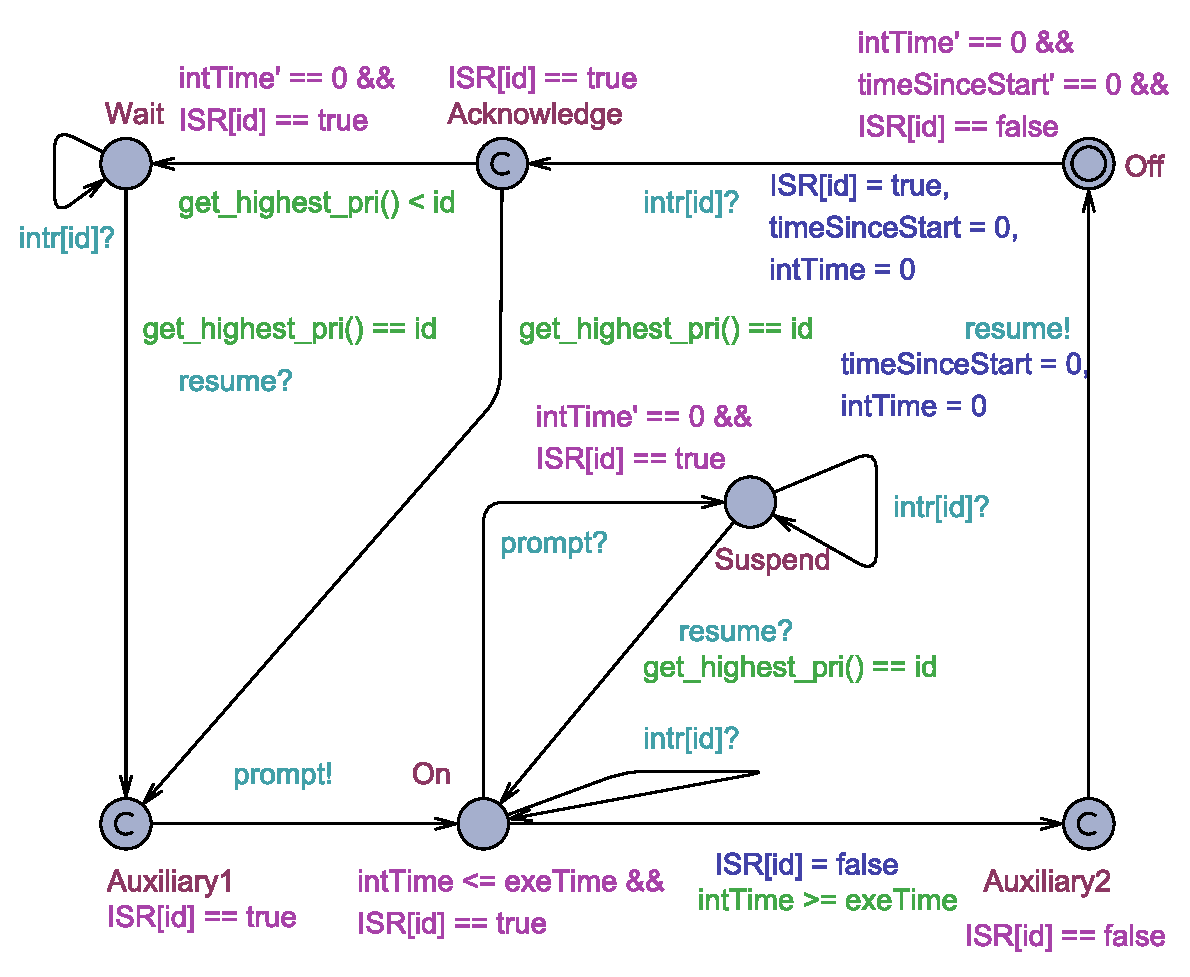
\includegraphics[width=0.8\textwidth]{Interrupt_basic}
	\caption{基本中断}
	\label{fig:interrupt_basic}
\end{figure}

\begin{longtabu} to \linewidth {p{5em}p{5em}XXXX}
	\caption{基本中断:变迁 }
	\label{tab:basic_intr_mov}\\
	\toprule[1.5pt]
	{\heiti 迁出位置} & {\heiti 迁入位置} & {\heiti 条件} & {\heiti 标签} & 
	{\heiti 变量修改} & {\heiti 含义}\\
	\midrule[1pt]
	\endfirsthead
	\multicolumn{6}{c}{续表~\thetable\hskip1em 基本中断模板:变迁}\\
	\toprule[1.5pt]
	{\heiti 迁出位置} & {\heiti 迁入位置} & {\heiti 条件} & {\heiti 标签} & 
	{\heiti 变量修改} & {\heiti 含义}\\
	\midrule[1pt]
	\endhead
	\hline
	\multicolumn{6}{r}{续下页}
	\endfoot
	\endlastfoot
	Off & Acknowledge & & intr[id]? & ISR对应位置位,时钟清零 & 中断控
	制器接收到中断信号\\
	\midrule[0.5pt]
	Acknowledge & Wait & 本中断优先级不是最高 & & & 优先级不是最高,本中断等待\\
	\midrule[0.5pt]
	Wait & Auxiliary1 & 本中断优先级最高 & resume? & &  高优先级的中断执行完
	毕,本中断得到CPU\\
	\midrule[0.5pt]
	Wait & Wait & & intr[id]? & & 忽略本中断的其他实例\\
	\midrule[0.5pt]
	Acknowledge & Auxiliary1 & 本中断优先级最高 & & & 本中断优先级最高,准备
	执行\\
	\midrule[0.5pt]
	Auxiliary1 & On & & prompt! & & 当前中断获得CPU,打断其他正在被处
	理的中断\\
	\midrule[0.5pt]
	On & Suspend & & prompt? & & 当前中断被更高优先级的中断打断\\
	\midrule[0.5pt]
	On & On & & intr[id]? & & 忽略本中断的其他实例\\
	\midrule[0.5pt]
	Suspend & On & 本中断优先级最高 & resume? & & 高优先级的中断执行完毕,本
	中断得到CPU\\
	\midrule[0.5pt]
	Supend & Suspend & & intr[id]? & & 忽略本中断的其他实例\\
	\midrule[0.5pt]
	On & Auxiliary2 & 中断处理时间达到预设 & & ISR对应位复位 & 中断执行结束\\
	\midrule[0.5pt]
	Auxiliary2 & Off & & resume! & 时钟清零 & 通知其他中断获取CPU\\
	\bottomrule[1.5pt]
\end{longtabu}

对一个中断$\gamma=\gamma_r=(id, intTime, n)\in\varGamma$,因为$n$的取值会涉及
到自动机的位置及变迁,因此无法对一个参数化的$n$构造自动机。在此,我们取$n=3$,定
义变量current指示当前占有CPU的中断实例,并重新定义3个时钟intTime[3]分别刻画该中
断3个实例的执行时间。

\begin{figure}[H]
	\centering
	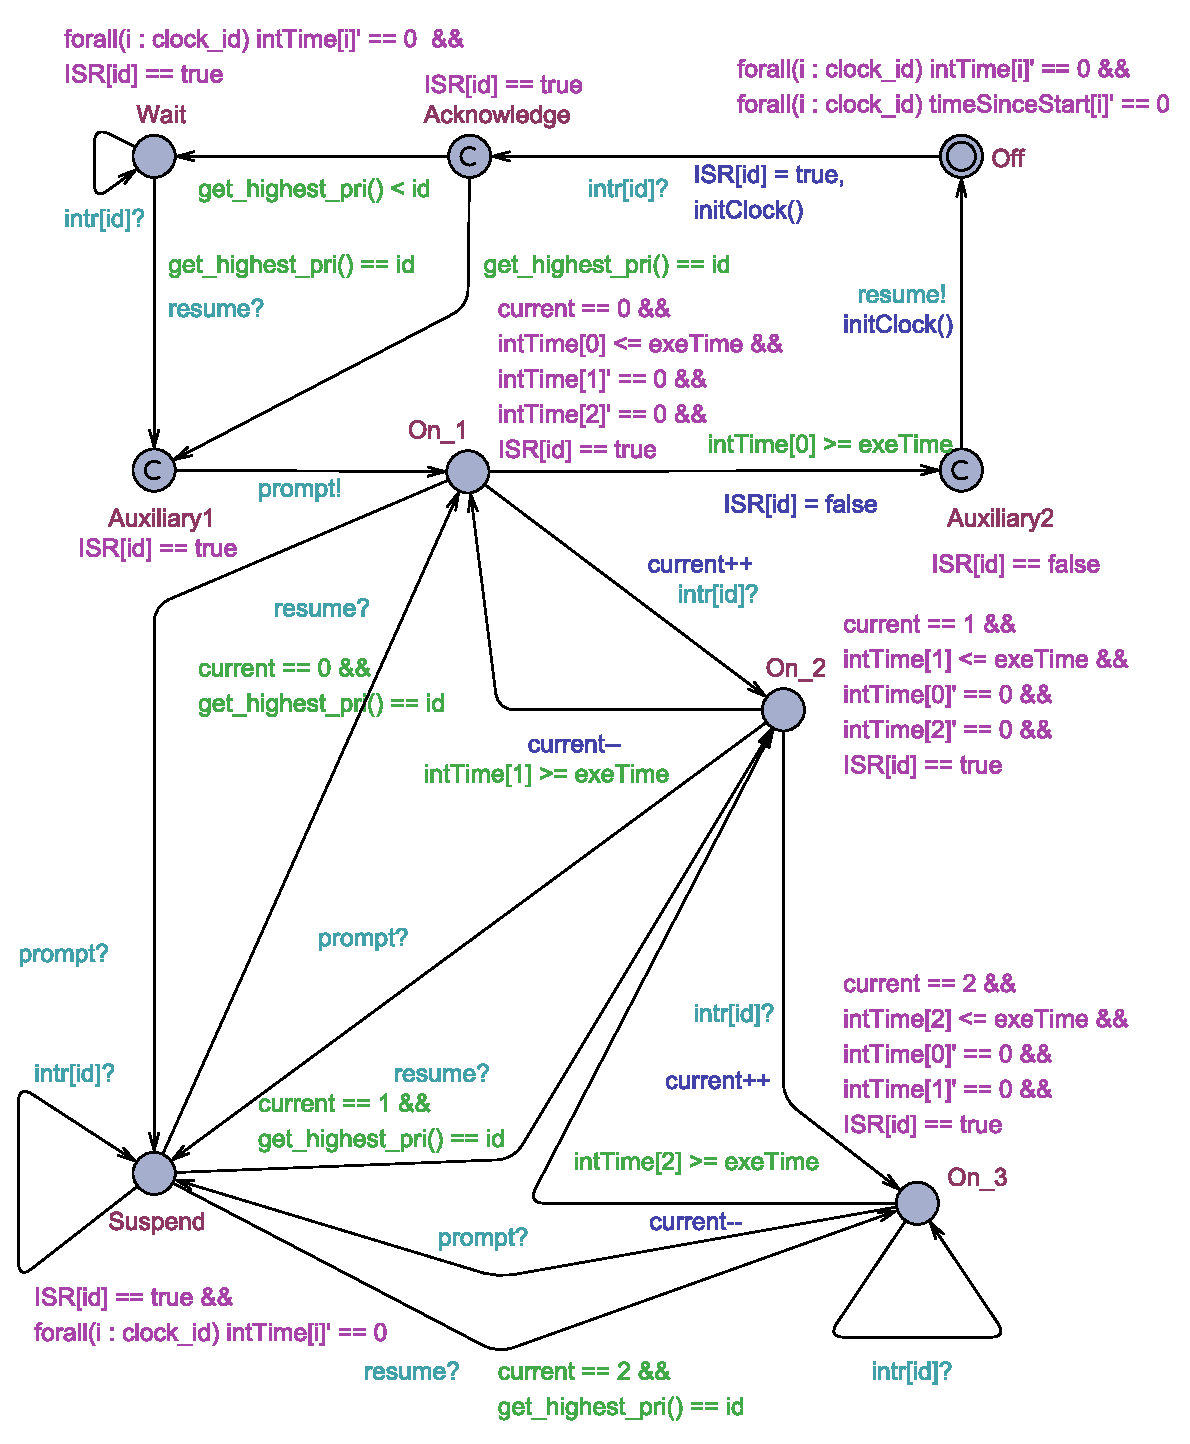
\includegraphics[width=\textwidth]{Interrupt_reentry}
	\caption{可重入中断}
	\label{fig:interrupt_reentrant}
\end{figure}

该自动机,相对于基本中断,最主要的区别就在于允许重入。由于重
入代表着新的示例,必然需要给每个实例分配一个时钟以记录其运行时间。同时,还需要一个
标记来表示当前的中断处于哪一个实例。因为在时间自动机网络的理论中,网络中的自动机
数量是固定的,在运行过程中不可变化。因此,在时间自动机网络运行过程中根据重入创建
新的自动机是不允许的。那么另一种思路就是将不同实例分别用各自的自动机来表示,模型
运行之前就全部构建好。这样做有一个问题,就是中断优先级的分配,这样必然导致需要在
网络中用一个共享变量还标示当前是哪个实例在运行,哪些实例在等待。否则,每次查找还
需要遍历所有的自动机网络,效率会很低。如果将网络展开,展开的自动机模型也会特别庞
大。另一种解决方案就是如本章所示,用一个自动机模型,并在其中分别用不同的位置标志
当前是哪个实例在运行。这样的好处显而易见,即不会破坏一个中断对应一个自动机的框架,
同时又能完美区分当前的实例。该时间自动机$\beta_r$如图~\ref{fig:interrupt_reentrant} 
所示。位置及变迁相关的定义参见表~\ref{tab:reentrant_intr_loc}和
表~\ref{tab:reentrant_intr_mov}。当$n$取其他值时,模型类似。


\begin{longtabu} to \linewidth {p{5em}p{5em}p{13em}X}
	\caption{可重入中断:位置}
	\label{tab:reentrant_intr_loc}\\
	\toprule[1.5pt]
	{\heiti 名称} & {\heiti 暂停时钟} & {\heiti 变量约束} & {\heiti 含义}\\
	\midrule[1pt]
	\endfirsthead
	\multicolumn{4}{c}{续表~\thetable\hskip1em 可重入中断:位置}\\
	\toprule[1.5pt]
	{\heiti 名称} & {\heiti 暂停时钟} & {\heiti 变量约束} & {\heiti 含义}\\
	\midrule[1pt]
	\endhead
	\hline
	\multicolumn{4}{r}{续下页}
	\endfoot
	\endlastfoot
	Off & intTime时钟组,timeSinceStart & ISR对应位为false & 初始位置,当前没
	有该中断\\
	\midrule[0.5pt]
	Acknowledge & 所有时钟 & ISR对应位为true & 中断控制器接收到中断信号\\
	\midrule[0.5pt]
	Wait & intTime时钟组 & ISR对应位为true & 当前有优先级更高的中断
	在运行,本中断等待。\\
	\midrule[0.5pt]
	Auxiliary1 & 所有时钟 & ISR对应位为true & 为表达Wait和Acknowledge到On\_1
	的语义设置的辅助位置\\
	\midrule[0.5pt]
	On\_1 & intTime[1], intTime[2] & intTime[0]不超过exeTime,ISR对应位为true & 
	中断正在被处理 \\
	\midrule[0.5pt]
	On\_2 & intTime[0], intTime[1] & intTime[1]不超过exeTime,ISR对应位为true & 
	中断被重入一次,正在被处理 \\
	\midrule[0.5pt]
	On\_3 & intTime[0], intTime[1] & intTime[2]不超过exeTime,ISR对应位为true & 
	中断被重入两次,正在被处理 \\
	\midrule[0.5pt]
	Suspend & intTime & ISR对应位为true & 中断被更高优先级抢占CPU \\ 
	\midrule[0.5pt]
	Auxiliary2 & 所有时钟 & ISR对应位为false & 为表达On\_1到Off的完整语义设置
	的辅助位置\\
	\bottomrule[1.5pt]
\end{longtabu}

\begin{longtabu} to \linewidth {p{5em}p{5em}XXXX}
	\caption{可重入中断:变迁 }
	\label{tab:reentrant_intr_mov}\\
	\toprule[1.5pt]
	{\heiti 迁出位置} & {\heiti 迁入位置} & {\heiti 条件} & {\heiti 标签} & 
	{\heiti 变量修改} & {\heiti 含义}\\
	\midrule[1pt]
	\endfirsthead
	\multicolumn{6}{c}{续表~\thetable\hskip1em 可重入中断:变迁}\\
	\toprule[1.5pt]
	{\heiti 迁出位置} & {\heiti 迁入位置} & {\heiti 条件} & {\heiti 标签} & 
	{\heiti 变量修改} & {\heiti 含义}\\
	\midrule[1pt]
	\endhead
	\hline
	\multicolumn{6}{r}{续下页}
	\endfoot
	\endlastfoot
	Off & Acknowledge & & intr[id]? & ISR对应位置位,时钟清零 & 中断控制器接
	收到中断信号\\
	\midrule[0.5pt]
	Acknowledge & Wait & 本中断优先级不是最高 & & & 当前有更高优先级的中断存
	在,本中断等待\\
	\midrule[0.5pt]
	Wait & Auxiliary1 & 本中断优先级最高 & resume? & &  高优先级的中断执行完毕,
	本中断得到CPU\\
	\midrule[0.5pt]
	Wait & Wait & & intr[id]? & & 忽略本中断的其他实例\\
	\midrule[0.5pt]
	Acknowledge & Auxiliary1 & 本中断优先级最高 & & & 本中断优先级最高,准备
	执行\\
	\midrule[0.5pt]
	Auxiliary1 & On\_1 & & prompt! & & 当前中断获得CPU,打断其他正在被处
	理的中断\\
	\midrule[0.5pt]
	On\_1 & Suspend & & prompt? & & 当前中断被更高优先级的中断打断\\
	\midrule[0.5pt]
	On\_1 & On\_2 & & intr[id]? & current增加1 & 发生第一次重入\\
	\midrule[0.5pt]
	On\_2 & Suspend & & prompt? & & 当前中断被更高优先级的中断打断\\
	\midrule[0.5pt]
	On\_2 & On\_3 & & intr[id]? & current增加1 & 发生第二次重入\\
	\midrule[0.5pt]
	On\_2 & On\_1 & intTime[1]达到exeTime & & current减少1 & 第一次重入处理完毕\\
	\midrule[0.5pt]
	On\_3 & Suspend & & prompt? & & 当前中断被更高优先级的中断打断\\
	\midrule[0.5pt]
	On\_3 & On\_3 & & intr[id]? &  & 忽略以后的本中断实例\\
	\midrule[0.5pt]
	On\_3 & On\_2 & intTime[2]达到exeTime & & current减少1 & 第二次重入处理完毕\\
	\midrule[0.5pt]
	Suspend & On\_1 & 本中断优先级最高 & resume? & & 高优先级的中断执
	行完毕,本中断得到CPU\\
	\midrule[0.5pt]
	Suspend & On\_2 & 本中断优先级最高 & resume? & & 高优先级的中断执
	行完毕,本中断得到CPU\\
	\midrule[0.5pt]
	Suspend & On\_3 & 本中断优先级最高 & resume? & & 高优先级的中断执
	行完毕,本中断得到CPU\\
	\midrule[0.5pt]
	Supend & Suspend & & intr[id]? & & 忽略本中断的其他实例\\
	\midrule[0.5pt]
	On\_1 & Auxiliary2 & intTime[0]达到exeTime & & ISR对应位复位 & 中断执行结束\\
	\midrule[0.5pt]
	Auxiliary2 & Off & & resume! & 时钟清零 & 通知其他中断获取CPU\\
	\bottomrule[1.5pt]
\end{longtabu}

对一个中断$\gamma=\gamma_s=(id, exeTime\_i, exeTime\_d)\in\varGamma$,构造该
自动机的难度在于,分段中断的第二段是在中断外的,因此要保证它在对应的位置将CPU让给
其他中断,同时又能在所有其他中断(如果分段中断则是他们前一段)执行结束之后取得CPU
继续执行。另外,在进入第二段之后,该执行仍然可以被打断,且恢复以后仍然需要回复到
该阶段。由此可见,分段中断的第一段和第二段是皆然不同的两种执行过程。因此我们需要
在自动机中描述这两种执行。其时间自
动机$\beta_s$如图~\ref{fig:interrupt_segment} 所示。位置及变迁相关的定义参见表
\ref{tab:sec_intr_loc}和表~\ref{tab:sec_intr_mov}。

\begin{figure}[H]
	\centering
	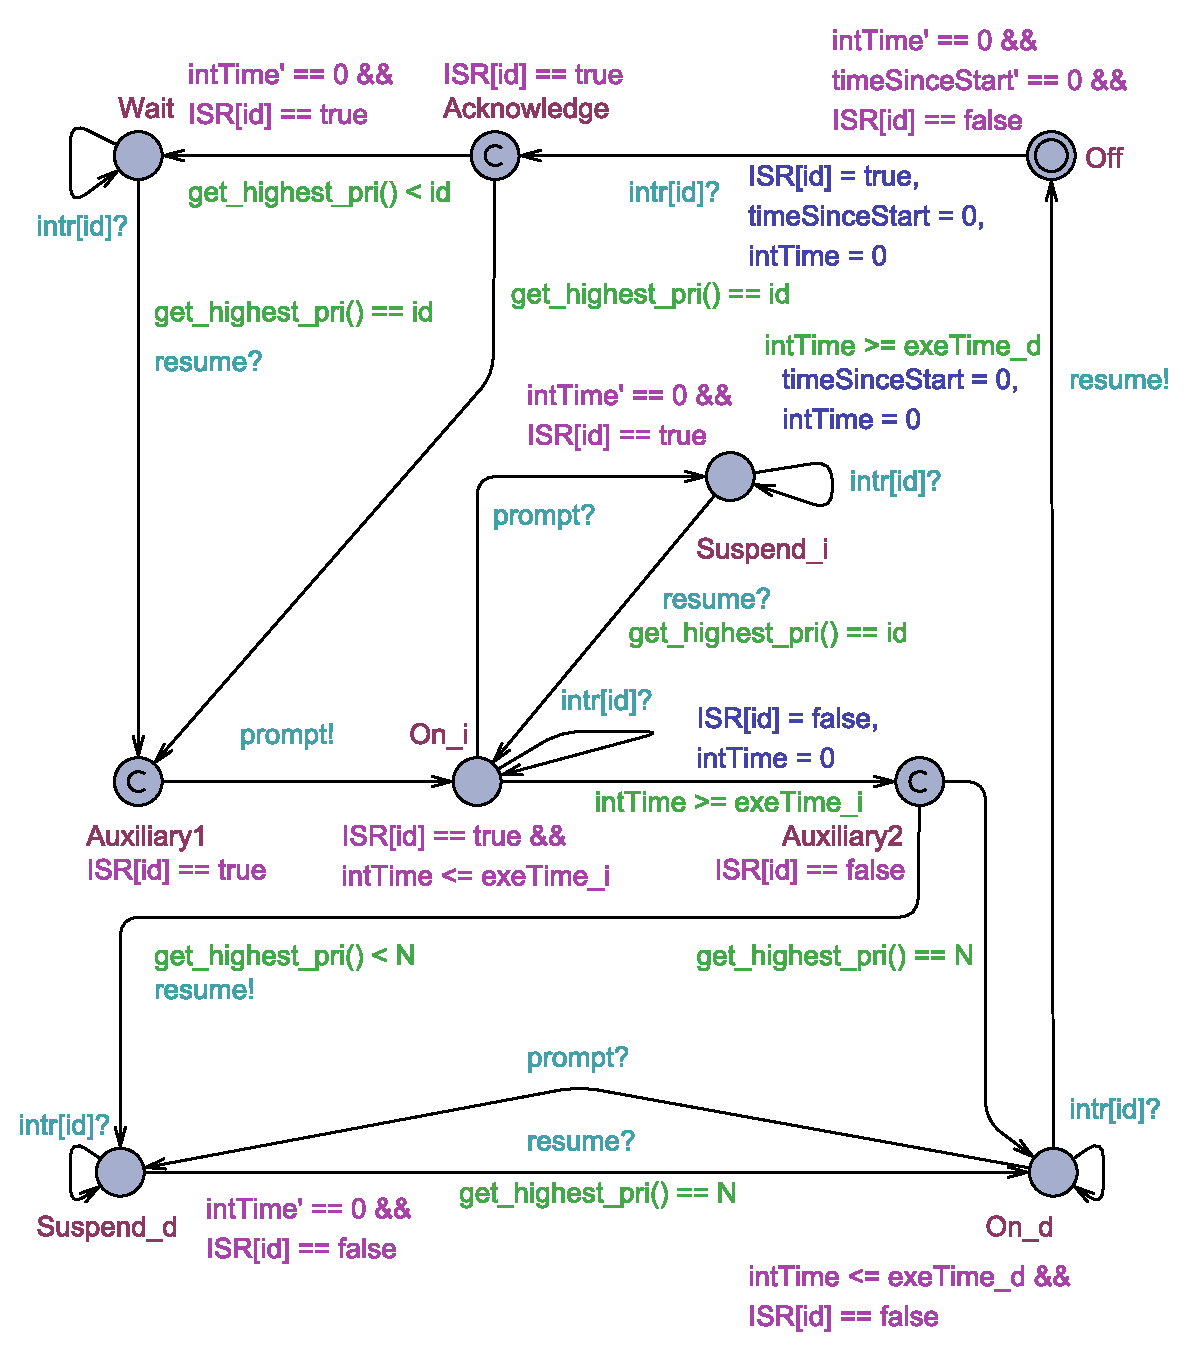
\includegraphics[width=\textwidth]{Interrupt_section}
	\caption{分段中断}
	\label{fig:interrupt_segment}
\end{figure}

\begin{longtabu} to \linewidth {p{5em}p{5em}p{13em}X}
	\caption{分段中断:位置}
	\label{tab:sec_intr_loc}\\
	\toprule[1.5pt]
	{\heiti 名称} & {\heiti 暂停时钟} & {\heiti 变量约束} & {\heiti 含义}\\
	\midrule[1pt]
	\endfirsthead
	\multicolumn{4}{c}{续表~\thetable\hskip1em 分段中断:位置}\\
	\toprule[1.5pt]
	{\heiti 名称} & {\heiti 暂停时钟} & {\heiti 变量约束} & {\heiti 含义}\\
	\midrule[1pt]
	\endhead
	\hline
	\multicolumn{4}{r}{续下页}
	\endfoot
	\endlastfoot
	Off & intTime和timeSinceStart & ISR对应位为false & 初始位置,当前没有
	该中断\\
	\midrule[0.5pt]
	Acknowledge & 所有时钟 & ISR对应位为true & 中断控制器接收中断信号\\
	\midrule[0.5pt]
	Wait & intTime & ISR对应位为true & 当前有优先级更高的中断在运行,本中断
	等待。\\
	\midrule[0.5pt]
	Auxiliary1 & 所有时钟 & ISR对应位为true & 为表达Wait和Acknowledge到On
	的语义设置的辅助位置\\
	\midrule[0.5pt]
	On\_i & & intTime不超过exeTime\_i,ISR对应位为true & 中断紧急处理分段
	正在被处理 \\
	\midrule[0.5pt]
	Suspend\_i & intTime & ISR对应位为true & 中断紧急处理分段被更高
	优先级的中断抢
	占CPU \\ 
	\midrule[0.5pt]
	Auxiliary2 & 所有时钟 & ISR对应位为false & 为表达On\_i到和On\_d和
	Suspend\_d的完整语义设置的辅助位置\\
	\midrule[0.5pt]
	On\_d & & intTime不超过exeTime\_d,ISR对应位为false & 中断推迟处理分
	段正在被处理 \\
	\midrule[0.5pt]
	Suspend\_d & intTime & ISR对应位为false & 中断推迟处理分段被抢
	占CPU \\ 
	\bottomrule[1.5pt]
\end{longtabu}

\begin{longtabu} to \linewidth {p{5em}p{5em}XXXX}
	\caption{分段中断:变迁 }
	\label{tab:sec_intr_mov}\\
	\toprule[1.5pt]
	{\heiti 迁出位置} & {\heiti 迁入位置} & {\heiti 条件} & {\heiti 标签} & 
	{\heiti 变量修改} & {\heiti 含义}\\
	\midrule[1pt]
	\endfirsthead
	\multicolumn{6}{c}{续表~\thetable\hskip1em 分段中断:变迁}\\
	\toprule[1.5pt]
	{\heiti 迁出位置} & {\heiti 迁入位置} & {\heiti 条件} & {\heiti 标签} & 
	{\heiti 变量修改} & {\heiti 含义}\\
	\midrule[1pt]
	\endhead
	\hline
	\multicolumn{6}{r}{续下页}
	\endfoot
	\endlastfoot
	Off & Acknowledge & & intr[id]? & ISR对应位置位,时钟清零 & 中断
	控制器接收到中断信号\\
	\midrule[0.5pt]
	Acknowledge & Wait & 本中断优先级不是最高 & & & 当前有更高优先级的中断
	存在,本中断等待\\
	\midrule[0.5pt]
	Wait & Auxiliary1 & 本中断优先级最高 & resume? & &  高优先级
	的中断执行完毕,本中断得到CPU\\
	\midrule[0.5pt]
	Wait & Wait & & intr[id]? & & 忽略本中断的其他实例\\
	\midrule[0.5pt]
	Acknowledge & Auxiliary1 & 本中断优先级最高 & & & 本中断优先级最高,
	准备\\
	\midrule[0.5pt]
	Auxiliary1 & On\_i & & prompt! & & 当前中断获得CPU,打断其他正
	在被处理的中断\\
	\midrule[0.5pt]
	On\_i & Suspend\_i & & prompt? & & 当前中断的紧急处理分段被
	更高优先级的中断打断\\
	\midrule[0.5pt]
	On\_i & On\_i & & intr[id]? & & 忽略本中断的其他实例\\
	\midrule[0.5pt]
	On\_i & Auxiliary2 & intTime达到exeTime\_i & & ISR对应位复位,intTime
	时钟清零 & 紧急处理分段完成,准备执行推迟处理分段\\
	\midrule[0.5pt]
	Suspend\_i & On\_i & 本中断优先级最高 & resume? & & 高优先级
	的中断执行完毕,本中断得到CPU\\
	\midrule[0.5pt]
	Supend\_i & Suspend\_i & & intr[id]? & & 忽略本中断的其他实例\\
	\midrule[0.5pt]
	Auxiliary2 & On\_d & 当前没有任何中断的紧急处理分段 & & & 开始执行推迟
	处理分段\\
	\midrule[0.5pt]
	Auxiliary2 & Suspend\_d & 当前有其他中断 & resume! & & 让出CPU\\
	\midrule[0.5pt]
	On\_d & Suspend\_d & & prompt? & & 其他中断触发,抢占CPU\\
	\midrule[0.5pt]
	On\_d & On\_d & & intr[id]? & & 忽略本中断的其他实例\\
	\midrule[0.5pt]
	On\_d & Off & intTime达到exeTime\_d & resume! & 所有时钟清零 & 
	本中断结束,让出CPU\\
	\midrule[0.5pt]
	Suspend\_d & On\_d & 当前没有任何中断的紧急处理分段 & resume? & & 所有中断的紧急
	处理分段结束\\
	\midrule[0.5pt]
	Suspend\_d & Suspend\_d & & intr[id]? & & 忽略本中断的其他实例\\
	\bottomrule[1.5pt]
\end{longtabu}

对中断系统$\Delta=(\varGamma, n)$中,$\gamma\in\varGamma$,$\gamma$在时间自动机网络
的自动机表示为$\beta$,有

\begin{equation}
	\beta := \beta_b~|~\beta_r~|~\beta_s
\end{equation}

对中断系统的时间自动机网络$NTA_\Delta$,则有

\begin{equation}
	NTA_\Delta := \beta_1~||~\beta_2~||\dots||~\beta_k, k = |\varGamma|
\end{equation}

\section{本章小结}
\label{sec:sum_3}

本章一开始提出了时间自动机理论分析嵌入式系统里中断实时性问题的一般方法。并且,按
照该方法,本章从现有研究相对深入透彻的多线程环境出发,立足于软硬件的实现细节,分
别对基本中断,可重入中断和分段中断归纳其行为模式,分析其实现原理。之后,本章在进
行合理抽象和假设的基础上,对上述三类中断分别给出了基于扩展的秒表自动机的形式化模
型,并给出了中断系统的时间自动机网络的定义。

本章构建的三类中断模型是从大量的文献阅读和项目实践中总结出的,涵盖了现有的绝大多
数中断。这些模型在应用到具体问题是可以作为已有的成果直接套用。在遇到一个不能简单
归结为这三类的中断时,也完全可以按照本章提出的方法,同时借鉴这三类中断时的思路来
完成模型构建。



